\documentclass[a4paper,10pt,twoside]{book}
\usepackage{a4wide}
\usepackage[english]{babel}
\usepackage{url}
\usepackage{verbatim}
\usepackage{tabularx}
\usepackage{ltxtable}


\usepackage{xcolor}
\usepackage{shadow}
\usepackage{ucs}
\usepackage[utf8x]{inputenc}
\usepackage[T1]{fontenc}
\usepackage{graphicx}
\usepackage{array}
\usepackage{verbatim}
\usepackage{tabularx}
\usepackage{ltxtable}
\usepackage{html}
\usepackage{tikz}
\usepackage{cmbright}

\definecolor{OFBlue}{HTML}{47617B}


\definecolor{Myorange}{cmyk}{0,0.42,1,0}
\definecolor{Myblue}{rgb}{0.2,0.2,1}
\definecolor{Mygrey}{gray}{0.85}


\definecolor{Myred}{rgb}{1,0.85,0.85}
\definecolor{Myblue}{rgb}{0.85,0.90,1}
\definecolor{Mygreen}{rgb}{0.4,1,0.4}

% whitecdp (formerly schulzrinne.sty) --provide for blank pages
% between chapters
% This redefinition of the \cleardoublepage command provides
% for a special pagestyle for the "extra" pages which are generated
% to ensure that the chapter opener is on a recto page.
% The pagestyle is "chapterverso"; for many publishers, this should be
% identical to "empty", so that's the default.
% \def\cleardoublepage{\clearpage
%  \if@twoside
%   \ifodd\c@page\else
%    \null\thispagestyle{chapterverso}\newpage
%    \if@twocolumn\null\newpage\fi
%    \fi
%   \fi
%  }%
% \def\ps@chapterverso{\ps@empty}%
\makeatletter
\def\cleardoublepage{\clearpage\if@twoside \ifodd\c@page\else
  \hbox{}
  \thispagestyle{empty}
  \newpage
  \if@twocolumn\hbox{}\newpage\fi\fi\fi}
\makeatother


% macro pour un exemple

% \newcommand{\exempleblock}[1]{
% \begin{latexonly}
% 	\begin{minipage}[t]{0.1\linewidth}
% 		\vspace{-0.5em}
% 	        \includegraphics[scale=0.17]{template/sigle_ex_code.png}
% 	\end{minipage}
% 	\colorbox{Mygrey}{
% 		\begin{minipage}[t]{0.83\linewidth}
% 			\vspace{0.2em}
% 			{{#1}}
% 		\end{minipage}
% 	}
% \end{latexonly}
% }


\newcommand{\coverpage}[3]{
\begin{titlepage}
  \begin{tikzpicture}[remember picture, overlay]
    \draw [fill=OFBlue] (-4,4) rectangle (-0.5,-29.7);
    \draw (7.8,-2.0) node {
\includegraphics[width=120mm]{common/graphics/openfluid.png}};
    \draw (16, -15) node [anchor=east] {\huge{\textbf{#1}}};
    \draw (16, -16) node [anchor=east] {\Large{\textbf{#2}}};
    \draw (1,-24) node [anchor=west] {
\includegraphics[width=50mm]{common/graphics/LISAH.png}};
    \draw (16,-24) node [anchor=east,text centered,text width=4cm]{\Large{\textit{#3}}};
 \end{tikzpicture}
\end{titlepage}

}




% \newcommand*\chapterlabel{}
% 
% \titleformat{\chapter}
% {\gdef\chapterlabel{}
%  \normalfont\sffamily\Huge\bfseries\scshape}
% {\gdef\chapterlabel{\thechapter\ }}{0pt}
% {\begin{tikzpicture}[remember picture,overlay]
%     \node[yshift=-3cm] at (current page.north west)
%       {\begin{tikzpicture}[remember picture, overlay]
%         \draw[fill=OFBlue] (0,0) rectangle
%           (\paperwidth,3cm);
%         \node[anchor=east,xshift=.9\paperwidth,rectangle,
%               rounded corners=20pt,inner sep=11pt,
%               fill=blue]
%               {\color{white} test};
%        \end{tikzpicture}
%       };
%    \end{tikzpicture}
% }
% \titlespacing*{\chapter}{0pt}{50pt}{-60pt}


\newcommand{\pfname}{OpenFLUID}


% macro pour du code

\newcommand{\codeblock}[1]{
\begin{latexonly}
	\begin{minipage}[t]{0.1\linewidth}
		\vspace{-0.5em}
%	        \includegraphics[scale=0.17]{template/sigle_ex_code.png}
	        \includegraphics[scale=0.8]{template/notecolor.png}
	\end{minipage}
	\colorbox{Mygrey}{
		\begin{minipage}[t]{0.83\linewidth}
			\vspace{0.2em}
			{\footnotesize{\texttt{#1}}\normalsize}
		\end{minipage}
	}
\end{latexonly}
}

\begin{htmlonly}
\renewcommand{\codeblock}[1]{
\begin{rawhtml}
<BR>
<TABLE WIDTH="100%" CELLPADDING="10"><TR><TD WIDTH="80" ALIGN="center" VALIGN="top">
\end{rawhtml}
\includegraphics[scale=1]{template/notecolor.png}
\begin{rawhtml}
</TD><TD BGCOLOR="#eeeeee" ALIGN="left" VALIGN="top">
\end{rawhtml}
	\texttt{#1}
\begin{rawhtml}
</TD></TR></TABLE><BR>
\end{rawhtml}

}
\end{htmlonly}


\newcommand{\codeblockfromfile}[1]{
	\begin{minipage}[t]{0.1\linewidth}
		\vspace{-0.5em}
%	        \includegraphics[scale=0.17]{template/sigle_ex_code.png}
	        \includegraphics[scale=0.8]{template/notecolor.png}
	\end{minipage}
	\colorbox{Mygrey}{
		\begin{minipage}[t]{0.83\linewidth}
			\vspace{0.2em}
			{\footnotesize\verbatiminput{#1}\normalsize}
		\end{minipage}
	}
}


\begin{htmlonly}
\renewcommand{\codeblockfromfile}[1]{
\begin{rawhtml}
<BR>
<TABLE WIDTH="100%" CELLPADDING="10"><TR><TD WIDTH="80" ALIGN="center" VALIGN="top">
\end{rawhtml}
\includegraphics[scale=1]{template/notecolor.png}
\begin{rawhtml}
</TD><TD BGCOLOR="#eeeeee" ALIGN="left" VALIGN="middle">
\end{rawhtml}
	\verbatiminput{#1}
\begin{rawhtml}
</TD></TR></TABLE><BR>
\end{rawhtml}

}
\end{htmlonly}

% % macro pour paragraphe A noter
% \newcommand{\noteblock}[1]{
% 	\hbox{\raisebox{-0.5em}{\vrule depth 0pt height 0.4pt width 1\linewidth}}
% 	\begin{minipage}[t]{0.1\linewidth}
% 		\vspace{-0.6em}
% 	        \includegraphics[scale=0.18]{template/sigle_a_noter.png}
% 	\end{minipage}
% 	\begin{minipage}[t]{0.86\linewidth}
% 		\vspace{0.em}
% 		{\sffamily{#1}}
% 	\end{minipage}
% 	\hbox{\raisebox{-0.2em}{\vrule depth 0pt height 0.4pt width 1\linewidth}}
% }

\newcommand{\noteblock}[1]{
\begin{latexonly}
	\begin{minipage}[t]{0.1\linewidth}
		\vspace{-0.5em}
%	        \includegraphics[scale=0.24]{template/sigle_a_noter.png}
	        \includegraphics[scale=0.8]{template/tipcolor.png}
	\end{minipage}
	\colorbox{Myblue}{
		\begin{minipage}[t]{0.83\linewidth}
			\vspace{0.2em}
			{\sffamily{#1}}
		\end{minipage}
	}
\end{latexonly}
}



\begin{htmlonly}
\renewcommand{\noteblock}[1]{
\begin{rawhtml}
<BR>
<TABLE WIDTH="100%" CELLPADDING="10"><TR><TD WIDTH="80" ALIGN="center" VALIGN="top">
\end{rawhtml}
\includegraphics[scale=1]{template/tipcolor.png}
\begin{rawhtml}
</TD><TD BGCOLOR="#E6F0FF" ALIGN="left" VALIGN="middle">
\end{rawhtml}
	\sffamily{#1}
\begin{rawhtml}
</TD></TR>
</TABLE><BR>
\end{rawhtml}

}
\end{htmlonly}



% macro pour paragraphe attention!
% \newcommand{\warnblock}[1]{
% 	\hbox{\raisebox{-0.5em}{\vrule depth 0pt height 0.4pt width 1\linewidth}}
% 	\begin{minipage}[t]{0.1\linewidth}
% 		\vspace{-0.6em}
% 	        \includegraphics[scale=0.24]{template/sigle_warn.png}
% 	\end{minipage}
% 	\begin{minipage}[t]{0.86\linewidth}
% 		\vspace{0.em}
% 		{\sffamily{#1}}
% 	\end{minipage}
% 	\hbox{\raisebox{-0.2em}{\vrule depth 0pt height 0.4pt width 1\linewidth}}
% }


% macro pour paragraphe attention!
\newcommand{\warnblock}[1]{
\begin{latexonly}
	\begin{minipage}[t]{0.1\linewidth}
		\vspace{-0.5em}
%	        \includegraphics[scale=0.24]{template/sigle_warn.png}
	        \includegraphics[scale=0.8]{template/warncolor.png}
	\end{minipage}
	\colorbox{Myred}{
		\begin{minipage}[t]{0.83\linewidth}
			\vspace{0.2em}
			{\sffamily{#1}}
		\end{minipage}
	}
\end{latexonly}
}


\begin{htmlonly}
\renewcommand{\warnblock}[1]{
\begin{rawhtml}
<BR>
<TABLE WIDTH="100%" CELLPADDING="10"><TR><TD WIDTH="80" ALIGN="center" VALIGN="top">
\end{rawhtml}
\includegraphics[scale=1]{template/warncolor.png}
\begin{rawhtml}
</TD><TD ALIGN="left" VALIGN="middle" BGCOLOR="#FFE6E6">
\end{rawhtml}
	\sffamily{#1}
\begin{rawhtml}
<BR></TD></TR>
</TABLE><BR>
\end{rawhtml}

}
\end{htmlonly}




\urlstyle{sf}




\begin{document}

\begin{latexonly}
\coverpage{Quickstart guide}{OpenFLUID-Engine 1.4.0}{Fabre, J.C., \linebreak and the modelling group at LISAH}
\end{latexonly}

\begin{htmlonly}
\begin{center}

\includegraphics[scale=1]{common/graphics/openfluid_html.png}
\end{center}
\end{htmlonly}

\setcounter{tocdepth}{1}
\tableofcontents

\chapter*{Foreword}
\addcontentsline{toc}{chapter}{Foreword}

This quick reference manual will help you to prepare and run simulations using
the OpenFLUID sofware. It will not explain the concepts behind the software, nor the
scientific approaches in landscape fluxes modelling and simulation. 

\section*{Typographic conventions}

\noindent The "to note" informations are emphasized like this:\\
\noteblock{
"to note" information with blue background...
}

\bigskip

\noindent The source code examples are emphasized like this:
\begin{lstlisting}[language=,title=\footnotesize\textit{example of source code}]
Source code, with grey background and fixed size font
\end{lstlisting}


\bigskip

\noindent The "warning" informations are emphasized like this:\\
\warnblock{
"warning" informations with red background...
}





\chapter{FluidX file(s) format}

This part of the manual describes the FluidX file(s) format. Refer to the "Usage"
part of this manual to run the simulation.

\section{Overview}

The FluidX file format is an XML based format for OpenFLUID input file(s).
The OpenFLUID input information can be provided by a one or many files using
the FluidX format.\\
Whatever the input information is put into one or many files, the following
sections must be defined in the input file set:
\begin{itemize}
  \item The \textit{model} section defined by the \texttt{<model>} tag
  \item The \textit{spatial domain} section defined by the \texttt{<domain>} tag
  \item The \textit{run configuration} section defined by the \texttt{<run>} tag
  \item The \textit{outputs configuration} section defined by the \texttt{<output>} tag  
\end{itemize}
The order of the sections is not significant. All of these sections must be
inclosed into an \textit{openfluid} section defined by the \texttt{<openfluid>}
tag.

\begin{lstlisting}[language=xml,title=\footnotesize\textit{summary view of the
XML tree for FluidX files}] <?xml version="1.0" standalone="yes"?>
<openfluid>

  <model>
    <!-- here is the model definition -->
  </model>

  <domain>
    <!-- here is the spatial domain definition, associated data and events -->   
  </domain>

  <output>
    <!-- here is the output configuration -->
  </output>

  <run>
    <!-- here is the run configuration -->
  </run>

</openfluid>
\end{lstlisting}


\section{Sections}


\subsection{Model}

The flux model is defined by an ordered set of data generators and simulations
functions that will be plugged to the \OFEname \ kernel. It defines the model
for the simulation. It can also include a global parameters section which
applies to all simulation functions and generators. The global parameters may
be overridden by local parameters of simulation functions or generators.\\
\noindent The flux model must be defined in a section delimited by the
\texttt{<model>} tag, and must be structured following these rules:
\begin{itemize}
  \item Inside the \texttt{<model>} tag, there must be a set of
  \texttt{<function>}, \texttt{<generator>} and \texttt{<gparams>} tags
  \item Each \texttt{<function>} tag must bring a \texttt{fileID} attribute giving
  the identifier of the simulation function; the value of the \texttt{fileID}
  attribute must match the file name (without extension) of a reachable and
  pluggable simulation function.
  \item Each \texttt{<function>} tag may include zero to many \texttt{<param>} tags giving
  parameters to the function. Each \texttt{<param>} tag must bring a \texttt{name} attribute giving
  the name of the parameter and a \texttt{value} attribute giving the value of the parameter. These parameters can be scalar or vector of integer values, floating point values, string values. In case of vector, the values of the vector are separated by a ; (semicolon).
  \item Each \texttt{<generator>} tag must bring a \texttt{varname} attribute giving 
  the name of the produced variable, a \texttt{unitclass} attribute giving the 
  unit class of the produced variable, a \texttt{method} attribute giving the 
  method used to produce the variable (\texttt{fixed} for constant value,
  \texttt{random} for random value in a range, \texttt{interp} for an
  interpolated value from given data series). An optional \texttt{<varsize>}
  attribute can be set in order to produce a vector variable instead of a scalar variable.
  \item Each \texttt{<generator>} tag may include zero to many \texttt{<param>}
  tags giving parameters to the generator. Each \texttt{<param>} tag must bring
  a \texttt{name} attribute giving the name of the parameter and a \texttt{value} 
  attribute giving the value of the parameter.
  \item A generator using the \texttt{fixed} method must provide a
  param named \texttt{fixedvalue} for the value to produce.
  \item A generator using the \texttt{random} method must provide a
  param named \texttt{min} and a param named \texttt{max} delimiting the
  random range for the value to produce.
  \item A generator using the \texttt{interp} method must provide a
  param named \texttt{sources} giving the data sources filename and a param
  named \texttt{distribution} giving the distribution filename for the value to
  produce (see appendix).
  \item Each \texttt{<gparams>} tag may include zero to many \texttt{<param>}
  tags giving the global parameters. Each \texttt{<param>} tag
  must bring a \texttt{name} attribute giving the name of the parameter and a \texttt{value} 
  attribute giving the value of the parameter.
\end{itemize}

\begin{lstlisting}[language=xml,title=\footnotesize\textit{example}]
<?xml version="1.0" standalone="yes"?>
<openfluid>
  <model>

    <gparams>
      <param name="gparam1" value="100" />
      <param name="gparam2" value="0.1" />
    </gparams>

    <function fileID="example.functionA" />

    <generator varname="example.generator.fixed" unitclass="EU1" method="fixed" varsize="11">
      <param name="fixedvalue" value="20" />
    </generator>

    <generator varname="example.generator.random" unitclass="EU2" method="random">
      <param name="min" value="20.53" />
      <param name="max" value="50" />
    </generator>

    <function fileID="example.functionB">
      <param name="param1" value="strvalue" />
      <param name="param2" value="1.1" />
      <param name="gparam1" value="50" />
    </function>

  </model>
</openfluid>
\end{lstlisting}

\warnblock{There must be only one model definition in the input dataset.}

\warnblock{The order of the simulation functions and data generators in the \texttt{<model>} section is very important : the same order will be used for execution on the same time step}


\bigskip

\subsection{Spatial domain}

\subsubsection{Definition and relationships}

The spatial domain is defined by a set of spatial units that are connected each others.
These spatial units are defined by a numerical identifier (ID) and a class.
They also include information about the processing order of the unit in the class.
Each unit can be connected to zero or many other units from the same or a different unit class.\\
\noindent The spatial domain definition must be defined in a section delimited
by the \texttt{<definition>} tag, which is a sub-section of the \texttt{domain}
tag, and must be structured following these rules:
\begin{itemize}
  \item Inside the \texttt{<definition>} tag, there must be a set of
  \texttt{<unit>} tags
  \item Each \texttt{<unit>} tag must bring an \texttt{ID} attribute giving
  the identifier of the unit, a \texttt{class} attribute giving the class of
  the unit, a \texttt{pcsorder} attribute giving the process order in the
  class of the unit
  \item Each \texttt{<unit>} tag may include zero or many \texttt{<to>} tags giving
  the outgoing connections to other units. Each \texttt{<to>} tag must bring an
  \texttt{ID} attribute giving the identifier of the connected unit and a
  \texttt{class} attribute giving the class of the connected unit
  \item Each \texttt{<unit>} tag may include zero or many \texttt{<childof>}
  tags giving the parent units. Each \texttt{<childof>} tag must bring an
  \texttt{ID} attribute giving the identifier of the parent unit and a
  \texttt{class} attribute giving the class of the parent unit   
\end{itemize}

\begin{lstlisting}[language=xml,title=\footnotesize\textit{example}]
<?xml version="1.0" standalone="yes"?>
<openfluid>
  <domain>
    <definition>

      <unit class="PU" ID="1" pcsorder="1" />

      <unit class="EU1" ID="3" pcsorder="1">
        <to class="EU1" ID="11" />
        <childof class="PU" ID="1" />
      </unit>
      
      <unit class="EU1" ID="11" pcsorder="3">
        <to class="EU2" ID="2" />
      </unit>
      
      <unit class="EU2" ID="2" pcsorder="1" />

    </definition>
  </domain>
</openfluid>
\end{lstlisting}
\bigskip


\subsubsection{Input data}

The spatial domain input data are static data brought by units, usually properties and initial conditions for each unit.\\
\noindent The spatial domain input data must be defined in a section delimited
by the \texttt{<inputdata>} tag, which is a sub-section of the \texttt{domain}
tag, and must be structured following these rules:
\begin{itemize}
  \item The \texttt{<inputdata>} tag must bring a \texttt{unitclass}
  attribute giving the unit class to which input data must be attached, and a
  \texttt{colorder} attribute giving the order of the contained column-formatted
  data
  \item Inside the \texttt{<inputdata>} tag, there must be the input data as 
  row-column text. As a rule, the first column is the ID of the unit in the class
  given through the the \texttt{unitclass} attribute of \texttt{<inputdata>}
  tag, the following columns are values following the column order given
  through the \texttt{colorder} attribute of the \texttt{<inputdata>} tag.
  Values for the data can be real, integer or string.
\end{itemize}

\bigskip

\begin{lstlisting}[language=xml,title=\footnotesize\textit{example}]
<?xml version="1.0" standalone="yes"?>
<openfluid>
  <domain>
  
    <inputdata unitclass="EU1" colorder="indataA">
      3 1.1
      11 7.5
    </inputdata>

    <inputdata unitclass="EU2" colorder="indataB1;indataB3">
      2 18 STRVALX
    </inputdata>

  </domain>
</openfluid>
\end{lstlisting}


\bigskip

\noteblock{Old inputdata format, with \texttt{<columns>} and \texttt{<data>}
 tags are still useable. However, you are encouraged to use the new FluidX
 file format.}


\bigskip

\subsubsection{Discrete events}

The discrete events are events occuring on units, and that can be processed by simulation functions. 
\noindent The spatial events must be defined in a section delimited
by the \texttt{<calendar>} tag, which is a sub-section of the \texttt{domain}
tag, and must be structured following these rules:

\begin{itemize}
  \item Inside the \texttt{<calendar>} tag, there must be a set of \texttt{<event>} tags 
  \item Each \texttt{<event>} tag must bring a \texttt{unitID} and a 
  \texttt{unitclass} attribute giving the unit on which occurs the event, a 
  \texttt{date} attribute giving the date and time of the event. The date
  format must be "YYYY-MM-DD hh:mm:ss". The \texttt{<event>} tag may bring a
  \texttt{name} attribute and a a \texttt{category} attribute, but they are
  actually ignored.
  \item Each \texttt{<event>} tag may include zero to many \texttt{<info>} tags.
  \item Each \texttt{<info>} tag give information about the event and must
  bring a \texttt{key} attribute giving the name (the "key") of the info, and a
  \texttt{value} attribute giving the value for this key.
\end{itemize}  
  
\begin{lstlisting}[language=xml,title=\footnotesize\textit{example}]
<?xml version="1.0" standalone="yes"?>
<openfluid>
  <domain>
    <calendar>

      <event unitclass="EU1" unitID="11" date="1999-12-31 23:59:59">
        <info key="when" value="before" />
        <info key="where" value="1" />
        <info key="var1" value="1.13" />
        <info key="var2" value="EADGBE" />
      </event>
      <event unitclass="EU2" unitID="3" date="2000-02-05 12:37:51">
        <info key="var3" value="152.27" />
        <info key="var4" value="XYZ" />
      </event>
      <event unitclass="EU1" unitID="11" date="2000-02-25 12:00:00">
        <info key="var1" value="1.15" />
        <info key="var2" value="EADG" />
      </event>

    </calendar>
  </domain>
</openfluid>
\end{lstlisting}
\bigskip

\subsection{Run configuration}

The configuration of the simulation gives the simulation period, the data
exchange time step, and the optionnal progressive output parameters.\\
\noindent The run configuration must be defined in a section delimited by the
\texttt{<run>} tag, and must be structured following these rules:
\begin{itemize}
  \item Inside the \texttt{<run>} tag, there must be a \texttt{<deltat>} tag
  giving the data exchange time step (in seconds)
  \item Inside the \texttt{<run>} tag, there must be a \texttt{<period>} tag
  giving the simulation period.
  \item The \texttt{<period>} tag must bring a \texttt{begin} and an
  \texttt{end} attributes, giving the dates of the beginning and the end of the
  simulation period. The dates formats for these attributes must be
  \texttt{YYYY-MM-DD hh:mm:ss}
  \item Inside the \texttt{<run>} tag, there may be a \texttt{<valuesbuffer>}
  tag for the number of time steps kept in memory. The number of step is given
  through a \texttt{steps} attribute. If not present, all values are kept in memory.
  \item Inside the \texttt{<run>} tag, there may be a \texttt{<filesbuffer>}
  tag for the size of the memory buffer for each file of results. The size is given
  in kilobytes through a \texttt{kbytes} attribute. If not present, the default value 
  is 2KB.

\end{itemize}

\begin{lstlisting}[language=xml,title=\footnotesize\textit{example}]
<?xml version="1.0" standalone="yes"?>
<openfluid>
  <run>

    <deltat>3600</deltat>
    <period begin="2000-01-01 00:00:00" end="2000-03-27 01:12:37" />
    
    <valuesbuffer steps="10" />
    <filesbuffer kbytes="8" />
    
  </run>
</openfluid>
\end{lstlisting}

\bigskip

\subsection{Outputs configuration}

The configuration of the simulation outputs gives the description of the saved
results.\\
\noindent The outputs configuration must be defined in a section delimited by
the \texttt{<output>} tag, and must be structured following these rules:
\begin{itemize}
  \item Inside the \texttt{<output>} tag, there must be one to many
  \texttt{<files>} tags, defining files formats for saved data.
  \item These \texttt{<files>} tags must bring a \texttt{colsep} attribute
  defining the separator strings between columns, a \texttt{dtformat} attribute
  defining the date time format used (it could be \texttt{6cols}, \texttt{iso}
  or user defined using strftime() format whis is described in the appendix
  part of this document), a \texttt{commentchar} attribute defining the string
  prefixing lines of comments in output files.
  \item Inside the \texttt{<files>} tags, there must be one to many
  \texttt{<set>} tags. Each \texttt{<set>} tag will lead to a set of files.
  \item Each \texttt{<set>} tag must bring a \texttt{name} attribute defining
  the name of the set (this will be used as a suffix for generated output
  files), a \texttt{unitsclass} attribute and a \texttt{unitsIDs} attribute
  defining the processed units, a \texttt{vars} attribute defining the
  processed variables. It may also bring an a \texttt{precision} attribute
  giving the number of significant digits for the values in the outputs files.
  The IDs for the \texttt{unitsIDs} attribute are semicolon-separated, the
  wildcard character ('*') can be used to include all units IDs for the given
  class. The variables names for the \texttt{vars} attribute are
  semicolon-separated, the wildcard character ('*') can be used to include all
  variables for the given class. The value for the \texttt{precision} attribute
  must be $\geq$ 0. If not provided, the default value for the precision is 5.
\end{itemize}


\begin{lstlisting}[language=xml,title=\footnotesize\textit{example}]
<?xml version="1.0" standalone="yes"?>
<openfluid>
  <output>

    <files colsep=" " dtformat="%Y %m %d %H %M %S" commentchar="%">     
      <set name="testRS" unitsclass="RS" unitsIDs="51;232" vars="*" />
      <set name="full" unitsclass="SU" unitsIDs="*" vars="*" precision="7"/>
    </files>  

  </output>
</openfluid>
\end{lstlisting}

\chapter{Usage information}

The \OFEname \ application is available on Linux, Windows and MacOSX platforms.
We encourage you to use \OFEname \ program on Linux platform as it is the
development and usually used platform.

\section{Installation}

On linux platforms, the \OFEname \ software is available as distribution
packages (deb, rpm) or archive files (tar.gz, tar.bz2). The recommanded way to
install it is to use packages for your Linux distribution. If you want to use
archive files, you have to unarchive the software according to the directory tree.\\
Once installed, the \texttt{openfluid-engine} command should be available.
You can check it by running the command \texttt{openfluid-engine}
\verb?--?\texttt{help} or \texttt{openfluid-engine} \verb?--?\texttt{version}
in your favorite terminal. You are now ready to run your first simulation.

\section{Input dataset}

Before running the simulation, the input dataset must be built.
An \OFEname \ input dataset includes different informations, defined in one or
many files:
\begin{itemize}
  \item the spatial domain definition
  \item the flux model definition
  \item the spatial domain input data 
  \item the discrete events
  \item the run configuration
  \item the outputs configuration
\end{itemize}

\noindent All files must be placed into any directory that can be reached by the
engine. The default searched directory is a directory named
\texttt{.openfluid/engine/OPENFLUID.IN} and located into the user home
directory (the user home directory may vary, depending on the used operating
system). This directory is not automatically created, it should be created by hand.
If you prefer to place your dataset in another directory, you can
specify it using command line options passed to the engine (\texttt{-i} or \verb?--?\texttt{input-dir}).\\

\noindent In order to build these files, we encouraged you to use a good text
editor or, better, an XML editor. You can also use custom scripts or macros in
specialized sotware, such as spreadsheets or Geographic Information Systems
(GIS), to generate automatically the input dataset.

\bigskip

% \section{Engine sequence}
% 
% The following sequence diagram describes the stage-by-stage execution of an
% \OFEname -engine simulation. The kernel is the main application, and the
% simulation function represents each simulation function used in the model definition.
% 
% \begin{latexonly}
% \begin{center}
% 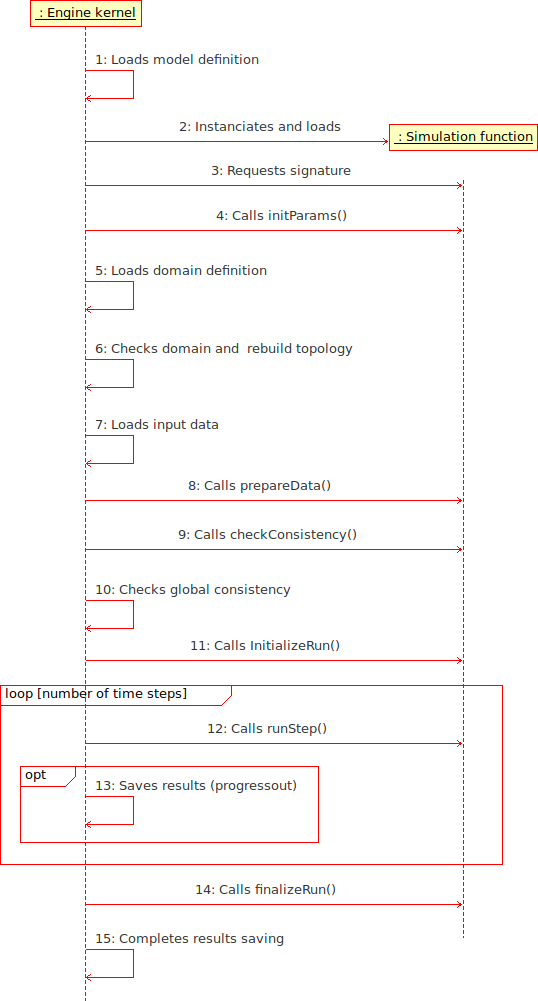
\includegraphics[scale=0.6]{common/graphics/ofeseq.png}
% \end{center}
% \end{latexonly}
% 
% \begin{htmlonly}
% \begin{center}
% 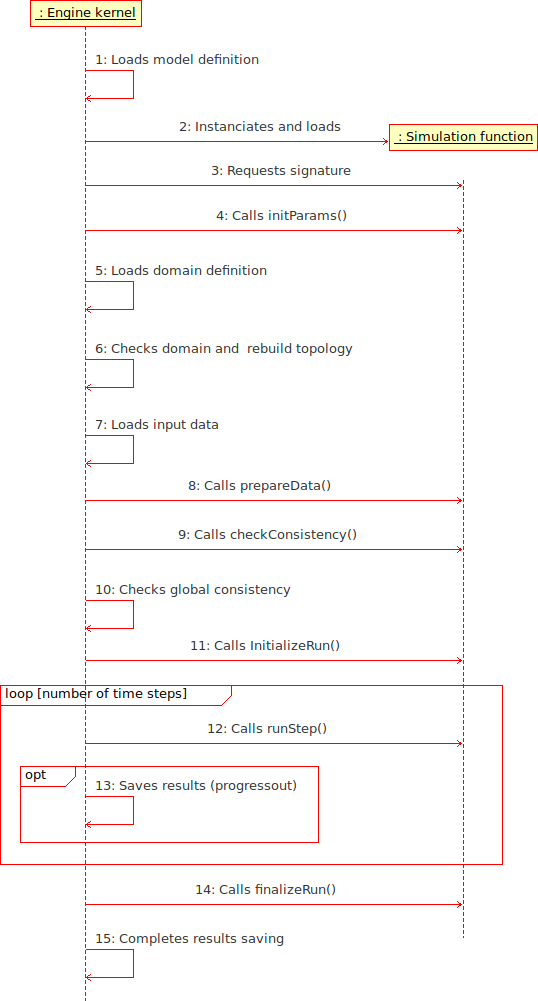
\includegraphics[scale=1]{common/graphics/ofeseq.png}
% \end{center}
% \end{htmlonly}
% 
% Stages description:
% \begin{enumerate}
%   \item the kernel loads the model definition (from the \texttt{model.xml} file)  
%   \item the kernel loads and instanciates the simulation functions, according to the model definition
%   \item the kernel requests the signature of each simulation function 
%   \item the kernel runs the initParams() method of each simulation function
%   \item the kernel loads the domain definition (from the \texttt{*.ddef.xml} files)
%   \item the kernel check the domain definition consistency and rebuild the domain topology
%   \item the kernel loads the domain input data (from the \texttt{*.ddata.xml} files)
%   \item the kernel runs the prepareData() method of each simulation function
%   \item the kernel runs the checkConsistency() method of each simulation function
%   \item the kernel checks the global consistency (model + domain definition + domain input data)
%   \item the kernel runs the initializeRun() method of each simulation function
%   \item at every time step, the kernel runs the runStep() method of each simulation function
%   \item at every time step, if the progressive output of results is enabled and if the current time step is a "progressive output time step", the kernel saves a packet of data and frees memory  
%   \item the kernel runs the finalizeRun() method of each simulation function
%   \item the kernel completes the save of results (all results if progressive output is disabled, the remaining results if progressive output is enabled) 
% \end{enumerate}
% 
% 
% \bigskip


\section{Run the simulation}

To run the simulation, if the dataset is located in the default searched directory, simply run the command \texttt{openfluid-engine} in your favorite terminal. 
To specify a different input dataset directory, use the \texttt{-i} or \verb?--?\texttt{input-dir} command line option.    

\bigskip

\begin{latexonly}
\begin{center}
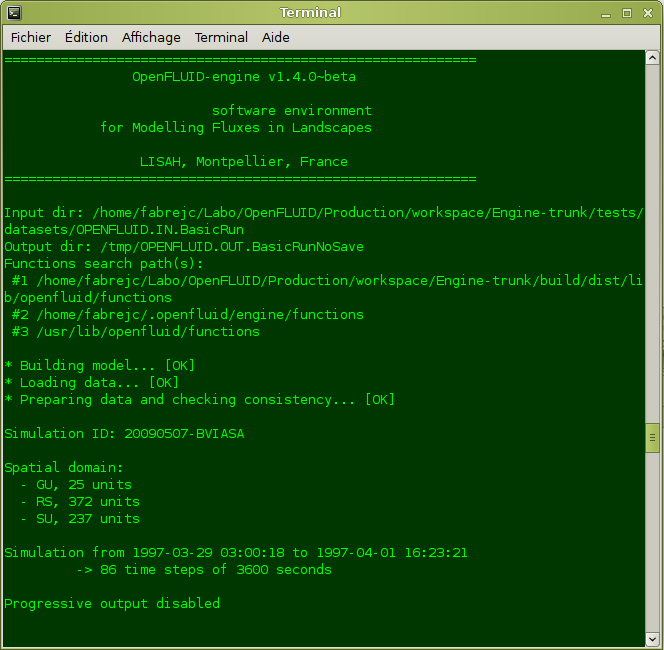
\includegraphics[scale=0.4]{common/graphics/oferun.png}
\end{center}
\end{latexonly}

\begin{htmlonly}
\begin{center}
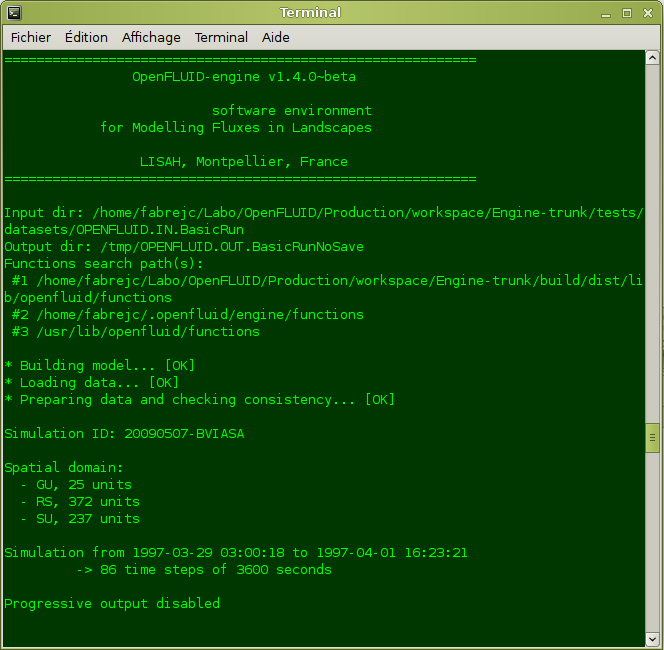
\includegraphics[scale=0.8]{common/graphics/oferun.png}
\end{center}
\end{htmlonly}

\section{Explore the results}

The results are stored in files, gathered by spatial unit. In each files, the
values for variables are stored as columns, each row corresponfing to a data
exchange time step (represented as a date and time). The format of the files
depends on the configuration of outputs, set through the \texttt{run.xml} file.
The default output directory is a directory named
\texttt{.openfluid/engine/OPENFLUID.OUT} and located into the user home
directory (the user home directory may vary, depending on the used operating
system). If you prefer to store your outputs into another directory, you can
specify it using command line options passed to the engine (\texttt{-o} or
\verb?--?\texttt{output-dir}).\\

\noindent In order to process the results of your simulations, we encourage you
to use software environments such as R, Scilab or Octave, spreadsheets such as
OpenOffice Calc, GIS such as GRASS or QGIS.

\section{Buddies}

Buddies are small tools that help scientific developers in order to complete
the modelling and/or development works. They are usable from the command line,
using the \verb?--?\texttt{buddyhelp}, \verb?--?\texttt{buddy} and
\verb?--?\texttt{buddyopts} options. Four buddies are available:
\begin{itemize}
  \item \texttt{func2doc}  
  \item \texttt{newfunc}
  \item \texttt{newdata}
  \item \texttt{convert}
\end{itemize}

\noindent Options are given to buddies through a comma-separated list of \texttt{key=value} arguments, using the \verb?--?\texttt{buddyopts} command line option.\\

\noindent General usage is:\\
\texttt{openfluid-engine --buddy buddyname --buddyopts abuddyopt=avalue,anotherbuddyopt=anothervalue}

\subsection{func2doc}

The \texttt{func2doc} buddy extracts scientific information from the source code
of simulation functions. It uses the function signature and \LaTeX-formatted text
placed between the \texttt{<func2doc>} and \texttt{</func2doc>} tags (usually
into C++ comments). From these sources of information, it builds a \LaTeX\
document which could be compiled into a PDF document and/or HTML pages.\\
The \texttt{func2doc} buddy can also use information from an optional
sub-directory named \texttt{doc}, located in the same directory as the input source file. The
information in the \texttt{doc} subdirectory should be linked to the information
from the source code using \LaTeX\ \texttt{\textbackslash input} command. The
\texttt{func2doc} buddy is available on UNIX only systems (Linux, MacOSX).

\bigskip

\noindent Required options:
\begin{center}
\begin{tabularx}{\linewidth}{lX}
\texttt{inputcpp}&path for cpp file to parse\\
\texttt{outputdir}&path for generated files\\
\end{tabularx}
\end{center}

\noindent Other options:
\begin{center}
\begin{tabularx}{\linewidth}{lX}
\texttt{html}&set to 1 in order to generate documentation as HTML files\\
\texttt{pdf}&set to 1 in order to generate documentation as PDF file\\
\texttt{tplfile}&path to template file\\
\end{tabularx}
\end{center}

\bigskip

\noindent Usage example:\\
\texttt{openfluid-engine --buddy func2doc --buddyopts
inputcpp=/path/to/cppfile.cpp, outputdir=/path/to/outputdir,pdf=1}


\subsection{newfunc}

The \texttt{newfunc} buddy generate a skeleton source code of a simulation
function, using given options.

\bigskip

\noindent Required options:
\begin{center}
\begin{tabularx}{\linewidth}{lX}
\texttt{cppclass}&C++ class name of the function\\
\texttt{funcid}&ID of the function\\
\end{tabularx}
\end{center}
    
\noindent Other options:
\begin{center}
\begin{tabularx}{\linewidth}{lX}
\texttt{authoremail}&email(s) of the author(s) of the function\\
\texttt{authorname}&name(s) of the author(s) of the function\\
\texttt{outputdir}&path for generated files\\
\end{tabularx}
\end{center}

\bigskip

\noindent Usage example:\\
\texttt{openfluid-engine --buddy newfunc --buddyopts
funcid=domain.subdomain.process.method, outputdir=/path/to/outputdir}


\subsection{newdata}

The \texttt{newdata} buddy generate a skeleton dataset. 

\bigskip

\noindent Required options:
\begin{center}
\begin{tabularx}{\linewidth}{lX}
\texttt{outputdir}&Output directory for generated dataset\\
\end{tabularx}
\end{center}

\bigskip

\noindent Usage example:\\
\texttt{openfluid-engine --buddy newdata --buddyopts
outputdir=/path/to/outputdir}

\subsection{convert}

The \texttt{convert} buddy converts a dataset from a specific version format to another one.
Currently, conversion is possible from 1.3.x format to 1.4.x format, and from 1.4.x format to 1.5.x format 

\bigskip

\noindent Required options:
\begin{center}
\begin{tabularx}{\linewidth}{lX} 
\texttt{convmode}&Conversion mode. Available modes are: \texttt{13\_14}, \texttt{13\_15}\\
\texttt{inputdir}&Input directory for dataset to convert\\ 
\texttt{outputdir}&Output directory for converted dataset\\
\end{tabularx}
\end{center}

\bigskip

\noindent Usage example:\\
\texttt{openfluid-engine --buddy convert --buddyopts convmode=13\_14,
inputdir=/path/to/inputdir,outputdir=/path/to/outputdir}



\chapter{Appendix}



\section{Command line options}

\begin{center}
\begin{tabularx}{\linewidth}{lX}
\texttt{-a}, \verb?---?\texttt{auto-output-dir}&generate automatic results output directory\\
\texttt{-b}, \verb?---?\texttt{buddy <arg>}&run specified OpenFLUID buddy\\
\verb?---?\texttt{buddyhelp <arg>}&display help message for specified OpenFLUID buddy\\
\verb?---?\texttt{buddyopts <arg>}&set options for specified OpenFLUID buddy\\
\texttt{-c}, \verb?---?\texttt{clean-output-dir}&clean results output directory by removing existing files\\
\texttt{-f}, \verb?---?\texttt{functions-list}&list available functions (do not run the simulation)\\
\texttt{-h}, \verb?---?\texttt{help}&display help message\\
\texttt{-i}, \verb?---?\texttt{input-dir <arg>}&set dataset input directory\\
\texttt{-k}, \verb?---?\texttt{enable-simulation-profiling}&enable time profiling for functions\\
\texttt{-o}, \verb?---?\texttt{output-dir <arg>}&set results output directory\\
\texttt{-p}, \verb?---?\texttt{functions-paths <arg>}&add extra functions research paths\\
\texttt{-q}, \verb?---?\texttt{quiet}&quiet display during simulation run\\
\texttt{-r}, \verb?---?\texttt{functions-report}&print a report of available functions, with details (do not run the simulation)\\
\texttt{-s}, \verb?---?\texttt{no-simreport}&do not generate simulation report\\
\verb?---?\texttt{show-paths}&print the used paths (do not run the simulation)\\
\texttt{-u}, \verb?---?\texttt{matching-functions-report <arg>}&print a report of functions matching the given wildcard-based pattern (do not run the simulation)\\
\texttt{-v}, \verb?---?\texttt{verbose}&verbose display during simulation\\
\verb?---?\texttt{version}&get version (do not run the simulation)\\
\texttt{-w}, \verb?---?\texttt{project <arg>}&set project directory\\
\texttt{-x}, \verb?---?\texttt{xml-functions-report}&print a report of available functions in xml format, with details (do not run the simulation)\\
\texttt{-z}, \verb?---?\texttt{no-result}&do not write results files\\
\end{tabularx}
\end{center}


\medskip


\section{Environment variables}

The \OFname \ framework takes into account the following environment
variables (if they are set):
\begin{itemize}
\item \texttt{OPENFLUID\_FUNCS\_PATH}: extra search paths for \OFname \ simulation functions. The path are separated by colon on UNIX systems, and by semicolon on Windows systems. 
\item \texttt{OPENFLUID\_INSTALL\_PREFIX}: overrides automatic detection of install path, useful on Windows systems.
\end{itemize}

\medskip

\section{Structure of an OpenFLUID project}

An OpenFLUID project can be run using OpenFLUID-Engine or OpenFLUID-Builder software.
It is a directory including:
\begin{itemize}
  \item a \texttt{.openfluidprj} file containing informations about the project,  
  \item an \texttt{IN} subdirectory containing the input dataset,
  \item an \texttt{OUT} subdirectory as the default output directory, containing the simulation results if any. 
\end{itemize}

The \texttt{.openfluidprj} contains the name of the project, the description of the project, the authors,
the creation date, the date of the latest modification, and a flag for
incremental output directory (this feature is currently disabled). 

\begin{lstlisting}[language=,title=\footnotesize\textit{example of .openfluidprj file}]
[OpenFLUID Project]
Name=a dummy project
Description=
Authors=John Doe
IncOutput=false
CreationDate=20110527T121530
LastModDate=20110530T151431
\end{lstlisting}

\medskip

For example, if you wish to run a simulation with \texttt{openfluid-engine}, using the project located in
\texttt{/absolute/path/to/workdir/a\_dummy\_project}, the command line to use is:\\
\texttt{openfluid-engine -w /absolute/path/to/workdir/a\_dummy\_project}\\

\medskip


\section{Date-time formats used in outputs configuration}

The output.xml file can use the ANSI strftime() standards formats for date time, through a format string. 
The format string consists of zero or more conversion specifications and ordinary characters.
A conversion specification consists of a \% character and a terminating conversion character that determines the conversion specification's behaviour.
All ordinary characters (including the terminating null byte) are copied unchanged into the array.

\bigskip

For example, the nineteenth of April, two-thousand seven, at eleven hours, ten minutes and twenty-five seconds formatted using different format strings:
\begin{itemize}
\item "\verb|%d/%m/%Y %H:%M:%S|" will give "\verb|19/04/2007 10:11:25|"
\item "\verb|%Y-%m-%d %H.%M|" will give "\verb|2007-04-19 10.11|"
\item "\verb|%Y\t%m\t%d\t%H\t%M\t%S|" will give "\verb|2007 04  19  10  11  25|"
\end{itemize}

\newpage 
\noindent List of available conversion specifications:
\begin{center}
\rowcolors[]{1}{gray!5}{gray!10}
\begin{tabularx}{\linewidth}{lX}
\rowcolor{gray!30}\textbf{Format} & \textbf{Description} \\\hline
\%a & locale's abbreviated weekday name. \\
\%A & locale's full weekday name. \\
\%b & locale's abbreviated month name. \\
\%B & locale's full month name. \\
\%c & locale's appropriate date and time representation. \\
\%C & century number (the year divided by 100 and truncated to an integer) as a decimal number [00-99]. \\
\%d & day of the month as a decimal number [01,31]. \\
\%D & same as \%m/\%d/\%y. \\
\%e & day of the month as a decimal number [1,31]; a single digit is preceded by a space. \\
\%h & same as \%b. \\
\%H & hour (24-hour clock) as a decimal number [00,23]. \\
\%I & hour (12-hour clock) as a decimal number [01,12]. \\
\%j & day of the year as a decimal number [001,366]. \\
\%m & month as a decimal number [01,12]. \\
\%M & minute as a decimal number [00,59]. \\
\%n & is replaced by a newline character. \\
\%p & locale's equivalent of either a.m. or p.m. \\
\%r & time in a.m. and p.m. notation; in the POSIX locale this is equivalent to \%I:\%M:\%S \%p. \\
\%R & time in 24 hour notation (\%H:\%M). \\
\%S & second as a decimal number [00,61]. \\
\%t & is replaced by a tab character. \\
\%T & time (\%H:\%M:\%S). \\
\%u & weekday as a decimal number [1,7], with 1 representing Monday. \\
\%U & week number of the year (Sunday as the first day of the week) as a decimal number [00,53]. \\
\%V & week number of the year (Monday as the first day of the week) as a decimal number [01,53]. If the week containing 1 January has four or more days in the new year, then it is considered week 1. Otherwise, it is the last week of the previous year, and the next week is week 1. \\
\%w & weekday as a decimal number [0,6], with 0 representing Sunday. \\
\%W & week number of the year (Monday as the first day of the week) as a decimal number [00,53]. All days in a new year preceding the first Monday are considered to be in week 0. \\
\%x & locale's appropriate date representation. \\
\%X & locale's appropriate time representation. \\
\%y & year without century as a decimal number [00,99]. \\
\%Y & year with century as a decimal number. \\
\%Z & timezone name or abbreviation, or by no bytes if no timezone information exists. \\
\%\% & character \%. \\
\end{tabularx}
\end{center}

\medskip

\section{Example of an input dataset as a single FluidX file}

\begin{lstlisting}[language=xml,frame=]
<?xml version="1.0" standalone="yes"?>
<openfluid>

  <model>
    <gparams>
      <param name="gparam1" value="100" />
      <param name="gparam2" value="0.1" />
    </gparams>
    <function fileID="example.functionA" />
    <generator varname="example.generator.fixed" unitclass="EU1"
               method="fixed" varsize="11">
      <param name="fixedvalue" value="20" />
    </generator>
    <generator varname="example.generator.random" unitclass="EU2" 
               method="random">
      <param name="min" value="20.53" />
      <param name="max" value="50" />
    </generator>
    <function fileID="example.functionB">
      <param name="param1" value="strvalue" />
      <param name="param2" value="1.1" />
      <param name="gparam1" value="50" />
    </function>
  </model>


  <domain>

    <definition>
      <unit class="PU" ID="1" pcsorder="1" />
      <unit class="EU1" ID="3" pcsorder="1">
        <to class="EU1" ID="11" />
        <childof class="PU" ID="1" />
      </unit>
      <unit class="EU1" ID="11" pcsorder="3">
        <to class="EU2" ID="2" />
      </unit>
      <unit class="EU2" ID="2" pcsorder="1" />
    </definition>

    <inputdata unitclass="EU1" colorder="indataA">
      3 1.1
      11 7.5
    </inputdata>
    
    <inputdata unitclass="EU2" colorder="indataB1;indataB3">
      2 18 STRVALX
    </inputdata>
    
    <calendar>
      <event unitclass="EU1" unitID="11" date="1999-12-31 23:59:59">
        <info key="when" value="before" />
        <info key="where" value="1" />
        <info key="var1" value="1.13" />
        <info key="var2" value="EADGBE" />
      </event>
      <event unitclass="EU2" unitID="3" date="2000-02-05 12:37:51">
        <info key="var3" value="152.27" />
        <info key="var4" value="XYZ" />
      </event>
      <event unitclass="EU1" unitID="11" date="2000-02-25 12:00:00">
        <info key="var1" value="1.15" />
        <info key="var2" value="EADG" />
      </event>
    </calendar>
    
  </domain>


  <run>
    <deltat>3600</deltat>
    <period begin="2000-01-01 00:00:00" end="2000-03-27 01:12:37" />
    <valuesbuffer steps="50" />
    <filesbuffer kbytes="8" />
  </run>


  <output>
    <files colsep=" " dtformat="%Y %m %d %H %M %S" commentchar="%">
      <set name="testRS" unitsclass="RS" unitsIDs="51;232" vars="*" />
      <set name="full" unitsclass="SU" unitsIDs="*" vars="*" precision="7" />
    </files>
  </output>

</openfluid>
\end{lstlisting}

\bigskip 

\section{File formats for \texttt{interp} or \texttt{inject} data generator}

\subsection{Sources}
The sources file format is an XML based format which defines a list of sources
files associated to an unique ID.\\
\noindent The sources must be defined in a section delimited by the
\texttt{<datasources>} tag, inside an \texttt{<openfluid>} tag and must be
structured following these rules:
\begin{itemize}
  \item Inside the \texttt{<datasources>} tag, there must be a set of
  \texttt{<filesource>} tags
  \item Each \texttt{<filesource>} tag must bring an \texttt{ID}
  attribute giving the identifier of source, and an \texttt{file}
  attribute giving the name of the file containing the source of data. The files
  must be placed in the input directory of the simulation.
\end{itemize}

\begin{lstlisting}[language=xml,title=\footnotesize\textit{example of a sources list file}]
<?xml version="1.0" standalone="yes"?>
<openfluid>
 
 <datasources>
    <filesource ID="1" file="source1.dat" />
    <filesource ID="2" file="source2.dat" />    
  </datasources>
  
</openfluid>
\end{lstlisting}

\bigskip
An associated source data file is a seven columns text file, containing a serie
of values in time. The six first columns are the date using the following format
\texttt{YYYY MM DD HH MM SS}. The 7$^{th}$ column is the value itself.

 \begin{lstlisting}[language=,title=\footnotesize\textit{example of a source data file}]
1999 12 31 12 00 00 -1.0
1999 12 31 23 00 00 -5.0
2000 01 01 00 30 00 -15.0
2000 01 01 00 40 00 -5.0
2000 01 01 01 30 00 -15.0
\end{lstlisting}


\subsection{Distribution}

A distribution file is a two column file associating a unit ID
(1$^{st}$column) to a source ID (2$^{nd}$column).
\begin{lstlisting}[language=,title=\footnotesize\textit{example of distribution file}] <?xml version="1.0" standalone="yes"?> 1 1
2 2
3 1
4 2
5 1
\end{lstlisting}




\section{Header types examples}

The following examples show output files for 2 variables (var1 and var2) extracted from a 6
hours simulation ran at a time step of an hour.


\subsection{\texttt{none}}

\begin{lstlisting}[language=,title=\footnotesize\textit{example of an output data file}]
2000-01-01 00:00:00;0.00000;1.00000 
2000-01-01 01:00:00;2.00000;3.00000
2000-01-01 02:00:00;4.00000;5.00000
2000-01-01 03:00:00;6.00000;7.00000
2000-01-01 04:00:00;8.00000;9.00000
2000-01-01 05:00:00;10.00000;11.00000
\end{lstlisting}


\subsection{\texttt{info}}

\begin{lstlisting}[language=,title=\footnotesize\textit{example of an output data file}]
% simulation ID: 20110905-VZIRXC
% file: TestUnits2_full-info.scalars.out
% date: 2011-Sep-05 10:23:17.394061
% unit: TestUnits #2
% scalar variables order (after date and time columns): var1 var2

2000-01-01 00:00:00;0.00000;1.00000 
2000-01-01 01:00:00;2.00000;3.00000
2000-01-01 02:00:00;4.00000;5.00000
2000-01-01 03:00:00;6.00000;7.00000
2000-01-01 04:00:00;8.00000;9.00000
2000-01-01 05:00:00;10.00000;11.00000
\end{lstlisting}


\subsection{\texttt{colnames-as-data}}

\begin{lstlisting}[language=,title=\footnotesize\textit{example of an output data file}]
datetime;var1;var2
2000-01-01 00:00:00;0.00000;1.00000 
2000-01-01 01:00:00;2.00000;3.00000
2000-01-01 02:00:00;4.00000;5.00000
2000-01-01 03:00:00;6.00000;7.00000
2000-01-01 04:00:00;8.00000;9.00000
2000-01-01 05:00:00;10.00000;11.00000
\end{lstlisting}

\subsection{\texttt{full}}

\begin{lstlisting}[language=,title=\footnotesize\textit{example of an output data file}]
% simulation ID: 20110905-VZIRXC
% file: TestUnits2_full-info.scalars.out
% date: 2011-Sep-05 10:23:17.394061
% unit: TestUnits #2
% scalar variables order (after date and time columns): var1 var2

datetime;var1;var2
2000-01-01 00:00:00;0.00000;1.00000 
2000-01-01 01:00:00;2.00000;3.00000
2000-01-01 02:00:00;4.00000;5.00000
2000-01-01 03:00:00;6.00000;7.00000
2000-01-01 04:00:00;8.00000;9.00000
2000-01-01 05:00:00;10.00000;11.00000
\end{lstlisting}


\medskip

\section{Useful links}

\subsection{OpenFLUID project}

\begin{itemize}
  \item OpenFLUID web site : \textcolor{blue}{\url{http://www.umr-lisah.fr/openfluid/}}  
  \item OpenFLUID web community : \textcolor{blue}{\url{http://www.umr-lisah.fr/openfluid/community/}}
  \item OpenFLUID on SourceSup (software forge): \textcolor{blue}{\url{https://sourcesup.cru.fr/projects/openfluid/}} 
\end{itemize}


\subsection{External tools}

\begin{itemize}
  \item Geany : \textcolor{blue}{\url{http://www.geany.org/}}
  \item Gnuplot : \textcolor{blue}{\url{http://www.gnuplot.info/}}
  \item GRASS GIS : \textcolor{blue}{\url{http://grass.itc.it/}}
  \item jEdit : \textcolor{blue}{\url{http://www.jedit.org/}}
  \item Octave : \textcolor{blue}{\url{http://www.gnu.org/software/octave/}}
  \item QGIS : \textcolor{blue}{\url{http://www.qgis.org/}}
  \item R : \textcolor{blue}{\url{http://www.r-project.org/}}
  \item Scilab : \textcolor{blue}{\url{http://www.scilab.org/}} 
\end{itemize}   



\end{document}